\section{Implementação em Simulink}

O circuito da Figura~\ref{fig:simcirc} foi construído em Simulink com a biblioteca Simscape Electrical, e o controle foi implementado aplicando diretamente as equações do projeto: os PI de corrente com \textit{feedforward} \eqref{eq:pi}, o \textit{droop} e o PI de tensão, o filtro de demanda e as referências de corrente \eqref{eq:refs}, com os ganhos da Tabela~\ref{tab:ganhos}. As razões cíclicas alimentam PWM de $f_s=20$ kHz com comandos complementares, e o degrau de carga é aplicado por um bloco do tipo degrau. Os casos da Tabela~\ref{tab:casos} são obtidos do mesmo modelo, variando a carga, as razões cíclicas, as condições iniciais e a habilitação de cada ramo, que mantém as duas chaves abertas quando desligado. As grandezas foram medidas nos últimos períodos de chaveamento, em valor médio e em ondulação pico a pico.

\begin{figure}[H]
\centering
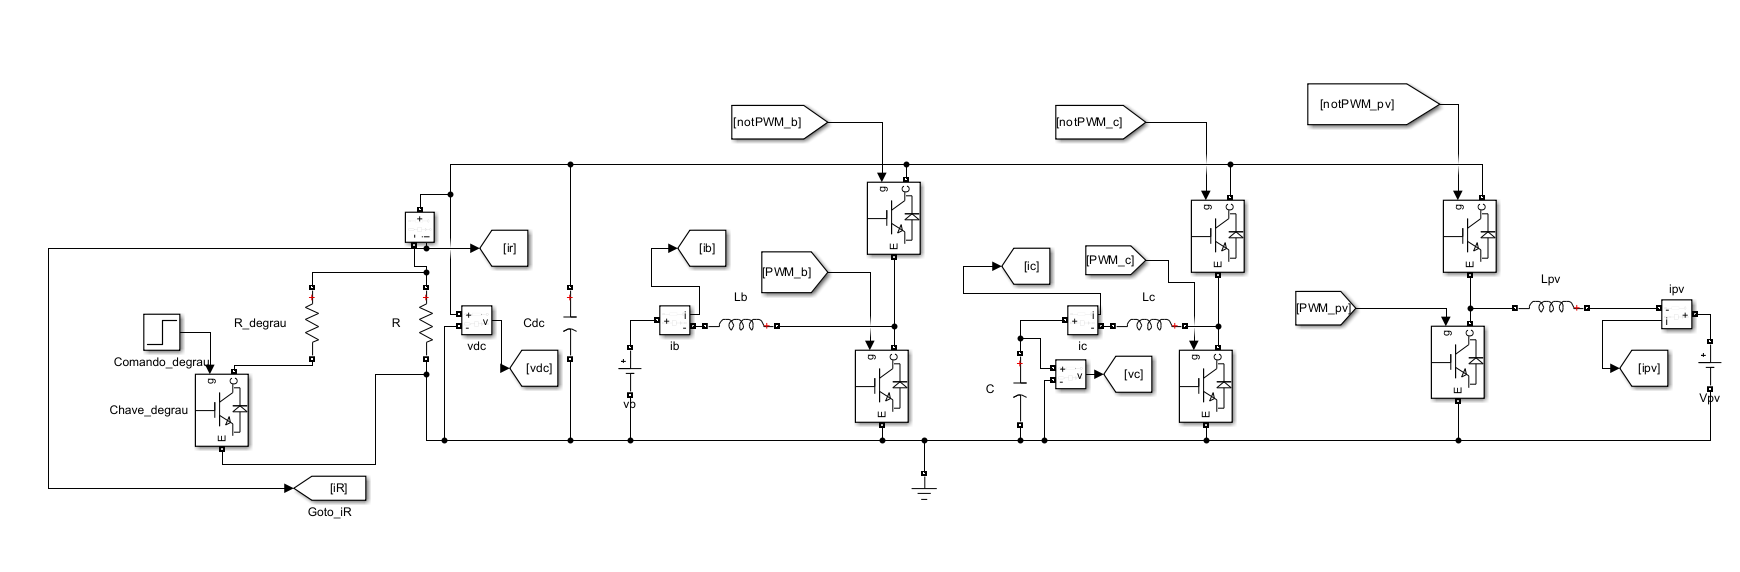
\includegraphics[width=\columnwidth]{images/fig_simulink_circuito.png}
\caption{Circuito implementado em Simulink.}
\label{fig:simcirc}
\end{figure}

\begin{figure}[H]
\centering
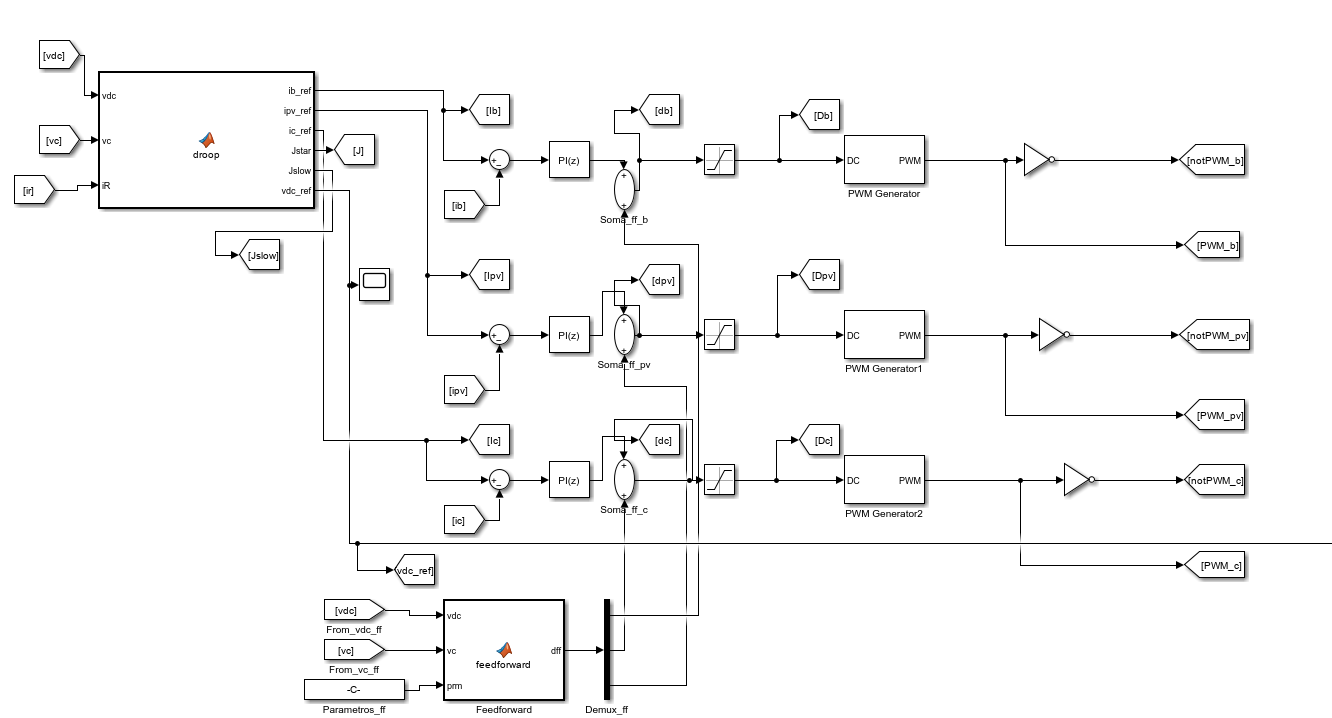
\includegraphics[width=\columnwidth]{images/fig_simulink_controle.png}
\caption{Subsistema de controle em Simulink.}
\label{fig:simctrl}
\end{figure}